\chapter{Les robots manipulateurs: définitions}
\label{sec:robotmanip}

Les robots manipulateurs correspondent à des bras artificiels, généralement plusieurs liens rigides connectés par des articulations. La grande majorité des robots industriels sont des robots manipulateurs qui ont comme tâche de positionner des outils pour la soudure, la peinture, etc. La figure \ref{fig:nom} présente les composants principaux d'un robot manipulateur. La figure \ref{fig:robotmanipex} illustre des exemples concrets de mécanismes et composants pour un robot manipulateur prototype. 

%%%%%%%%%%%%%%%%%%%%%%%%%%%%%%%%%%%%%%%%%%%%%%%%%%%%%%%%%%%%%%%%%%%%%%%%%%%%%
\begin{figure}[H]
	\centering
		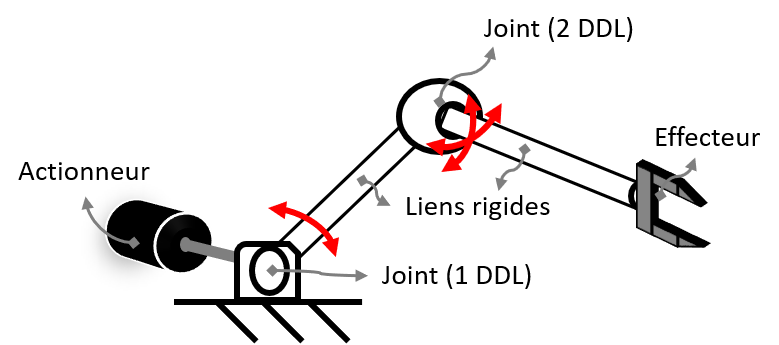
\includegraphics[width=0.55\textwidth]{nom.png}
	\caption{Nomenclature pour l'analyse d'un robot manipulateurs}
	\label{fig:nom}
\end{figure}
%%%%%%%%%%%%%%%%%%%%%%%%%%%%%%%%%%%%%%%%%%%%%%%%%%%%%%%%%%%%%%%%%%%%%%%%%%%%%%%

\section{Mécanismes et composants}

Cette section présente les différents composants d'un robot manipulateur ainsi que la nomenclature utilisée. 

\subsection{Liens rigides}

Un lien rigide d'un robot, c'est un ensemble de pièces fixes les unes par rapport aux autres qui forment un corps rigide. D'un point de vu de cinématique, deux pièces fixées de telle façon qu'aucun mouvement relatif n'est possible vont être considérées comme un seul lien. Par exemple, plusieurs tubes qui seraient soudés ensembles seraient considérés comme un seul lien rigide. 

\subsection{Joints (articulations)}

Les joints sont les articulations d'un robot. Un \textbf{joint prismatique} (articulation linéaire), permet la translation selon un axe entre deux pièces, et contraint les rotations relatives. Un \textbf{joint rotatif} (articulation angulaire), permet à deux pièces de pivoter relativement selon un axe. La variable $q_i$ utilisée pour décrire la configuration d'un joint $i$ est une distance pour un joint prismatique et un angle pour un joint rotatif.
%%%%%%%%%%%%%%%%%%%
\begin{align}
\text{Joint prismatique:} \quad q_i &= x_i      \quad [m] \\
\text{Joint rotatif    :} \quad q_i &= \theta_i \quad [rad]
\end{align} 
%%%%%%%%%%%%%%%%%%%

Les joints prismatiques et révolus ont une configuration décrite avec une seule variable, chacun des joints de ce type produit donc un degré de liberté (DDL) pour le robot manipulateur. Un robot utilisant seulement ces types de joints a donc un nombre total de DDL qui est égale au nombre de joints. Toutefois, des mécanismes plus complexes (ex.: joint sphérique comme illustré à la figure \ref{fig:nom}) peuvent produire plusieurs DDL en une seule articulation. Par contre, contrairement au corps humain, les robots utilisent généralement des joints prismatiques et rotatifs seulement pour simplifier la mécanique. Un joint sera dit actif si sa configuration est contrôlée par un actionneur, et passif si sa configuration est libre.
%%%%%%%%%%%%%%%%%%%%%%%%%%%%%%%%%%%%%%%%%%%%%%%%%%%%%%%%%%%%%%%
\begin{figure}[H]
				%\vspace{-10pt}
        \centering
        \subfloat[Joint prismatique]{
				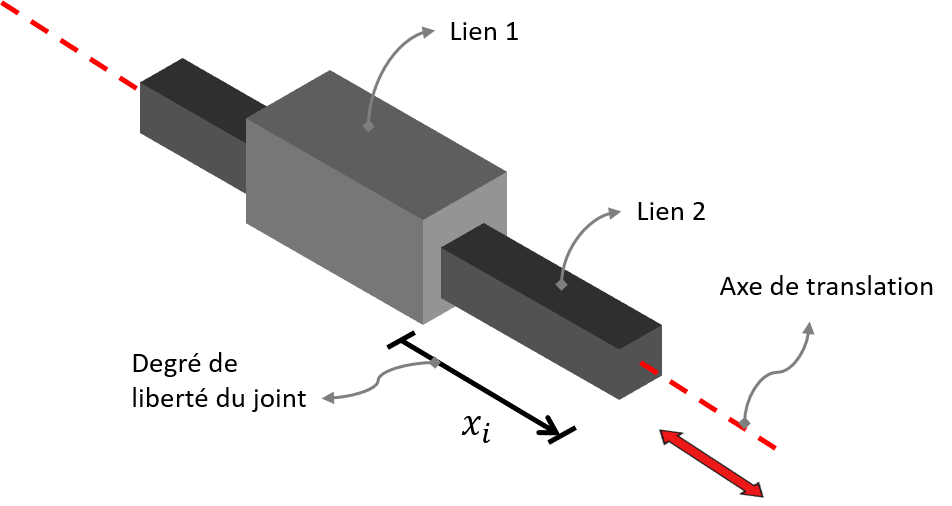
\includegraphics[width=0.48\textwidth]{jointpris}
				\label{fig:jointpris}}
				\subfloat[Joint rotatif]{
				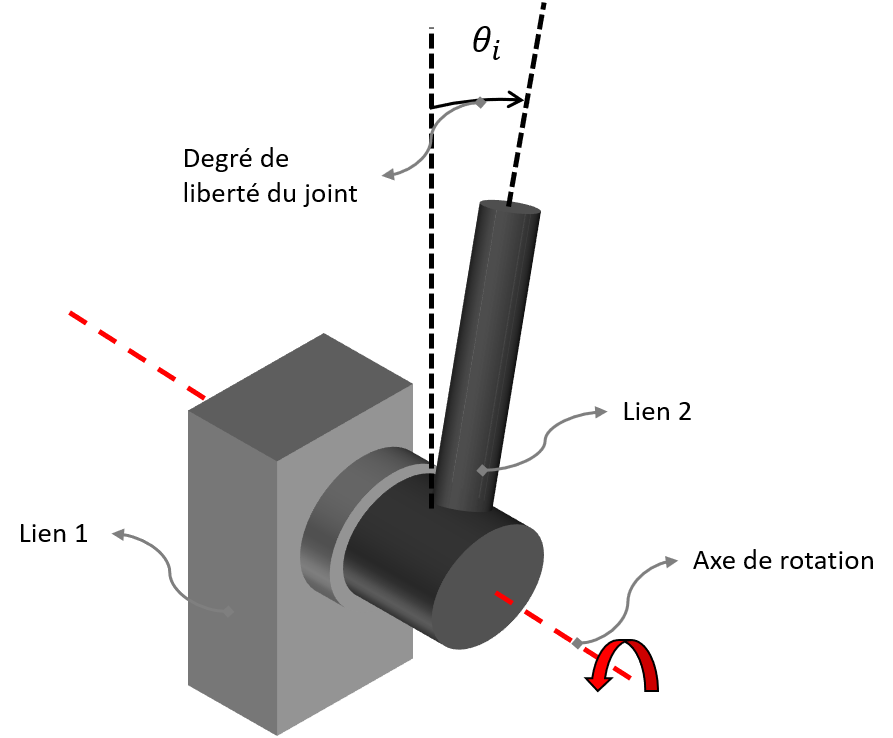
\includegraphics[width=0.48\textwidth]{jointrev}
				\label{fig:jointrev}}
        \caption{Joints à un degré de liberté}
				\label{fig:joint}
\end{figure}
%%%%%%%%%%%%%%%%%%%%%%%%%%%%%%%%%%%%%%%%%%%%%%%%%%%%%%%%%%%%%%%%%

\subsection{Effecteur}

L'effecteur est un terme générique qui réfère à la position de l'outil d'un robot manipulateur (ex.: une pince, une tête de soudure, une caméra, etc.). Dans un espace tri-dimensionnel, la position d'un objet nécessite au plus six variables pour être complètement décrite (voir section \ref{sec:corps}). L'effecteur d'un robot aura donc au plus 6 DDL. 

\subsection{Actionneurs}

Les actionneurs sont les muscles des bras robotiques. Un actionneur est fondamentalement un dispositif qui transforme de l'énergie en travail mécanique. La plupart des robots industriels utilisent des moteurs électriques pour actionner leurs joints, toutefois les actionneurs pourraient aussi être des vérins pneumatiques ou hydrauliques. 

\subsection{Capteurs}

Les capteurs sont les dispositifs qui collectent de l'information sur l'état interne d'un robot et/ou l’environnement. Pour la cinématique, les capteurs très régulièrement utilisés sont les encodeurs, qui mesurent directement la position des joints (variables $q_i$), et les systèmes de visions, qui mesurent la position de points dans le repère de la caméra. 


%%%%%%%%%%%%%%%
\begin{figure}[htbp]
	\centering
		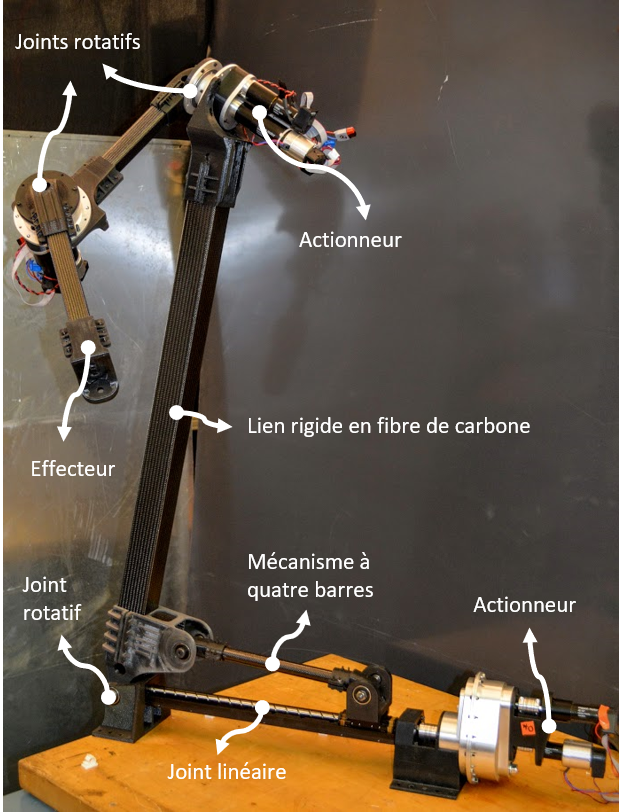
\includegraphics[width=0.80\textwidth]{robotmanipex.png}
	\caption{Prototype de robot manipulateur avec trois degrés de liberté}
	\label{fig:robotmanipex}
\end{figure}
%%%%%%%%%%%%%%%%%


\section{Configurations}

Cette section introduit les notions en lien avec la configuration d'un robot manipulateur.

\subsection{Degrés de liberté}

Le nombre de degrés de liberté (DDL), c'est le nombre de variables nécessaires pour complètement décrire la configuration d'un robot ou un mécanisme. La plupart des robots industriels ont six DDL, ce qui est suffisant pour pouvoir contrôler indépendamment les six DDL de l'effecteur. Pour des robots qui utilisent seulement des joints rotatifs comme illustré à la figure \ref{fig:ddl}, le nombre de DDL est égale au nombre de joints. Si le nombre de DDL est supérieur à six, le robot est dit \textbf{redondant}. Un robot redondant a plusieurs options de configuration des joints pour atteindre une position et une orientation désirées de l'effecteur. 

%%%%%%%%%%%%%%%%%%%%%%%%%%%%%%%%%%%%%%%%%%%%%%%%%%%%%%%%%%%%%%%
\begin{figure}[H]
				%\vspace{-10pt}
        \centering
        \subfloat[1 DDL]{
				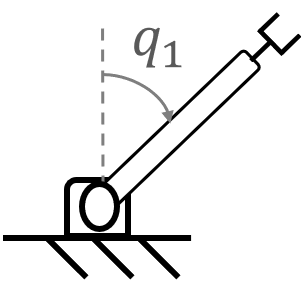
\includegraphics[width=0.20\textwidth]{1ddl}
				\label{fig:1ddl}}
				\subfloat[2 DDL]{
				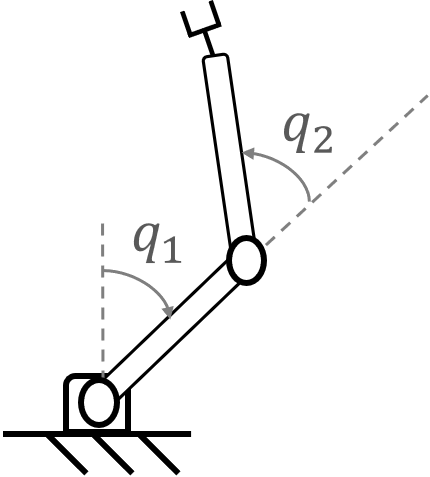
\includegraphics[width=0.25\textwidth]{2ddl}
				\label{fig:2ddl}}
				\subfloat[3 DDL]{
				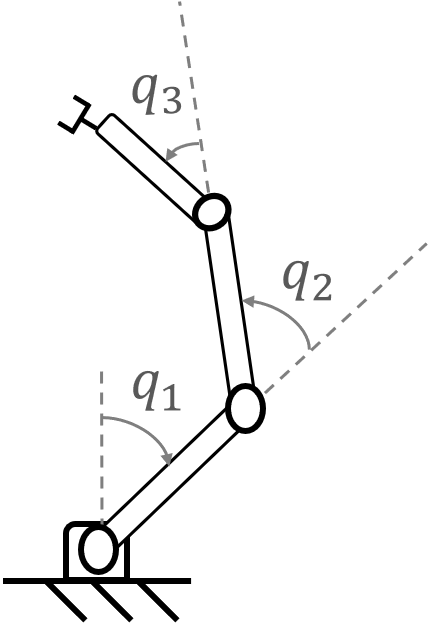
\includegraphics[width=0.25\textwidth]{3ddl}
				\label{fig:3ddl}}
        \caption{Manipulateurs planaires avec des joints rotatifs}
				\label{fig:ddl}
\end{figure}
%%%%%%%%%%%%%%%%%%%%%%%%%%%%%%%%%%%%%%%%%%%%%%%%%%%%%%%%%%%%%%%%%

\subsection{Espace de travail}

L'espace de travail c'est le volume qui comprend toutes les positions atteignables par l'effecteur du robot. La figure \ref{fig:workspace} illustre un espace de travail dans le plan d'un robot à deux joints. Parfois, des sous-ensembles de l'espace de travail peuvent être définis en fonction des positions atteignables avec une orientation précise de l'effecteur.

%%%%%%%%%%%%%%%%%%%%%%%%%%%%%%%%%%%%%%%%%%%%%%%%%%%%%%%%%%%%%%%%%%%%%%%%%%%%%
\begin{figure}[H]
	\centering
		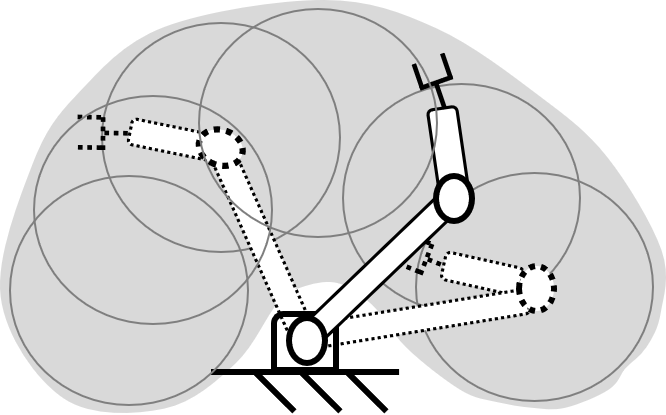
\includegraphics[width=0.45\textwidth]{workspace.png}
	\caption{Exemple de l'espace de travail d'un robot manipulateur à deux joints}
	\label{fig:workspace}
\end{figure}
%%%%%%%%%%%%%%%%%%%%%%%%%%%%%%%%%%%%%%%%%%%%%%%%%%%%%%%%%%%%%%%%%%%%%%%%%%%%%%%

%Parfois, des sous-ensembles de l'espace de travail 


%\subsection{Serie vs parallele}




\subsection{Configurations classiques}  

À venir!

%scara: https://www.youtube.com/watch?v=vKD20BTkXhk

